\documentclass[aspectratio=169]{beamer}

\usepackage[utf8]{inputenc}
\usepackage[russian]{babel}
\usepackage[T2A, T1]{fontenc}
\usefonttheme{serif}
\usetheme{Berkeley}
\usecolortheme{seagull}

\usepackage{fontspec}  
\setmainfont{Times New Roman} 
\setmonofont{Courier New}
\logo{\includegraphics[scale=0.5]{eltech-black-logo.eps}}

\addtobeamertemplate{navigation symbols}{}{%
	\usebeamerfont{footline}%
	\usebeamercolor[fg]{footline}%
	\hspace{1em}%
	\small
	\bfseries
	\insertframenumber/\inserttotalframenumber
}
\usepackage{listings}
\usepackage{tabularx}
\usepackage{multirow}
\usepackage{graphicx}
\usepackage{color, colortbl}
\definecolor{LightCyan}{rgb}{0.88,1,1}
\usepackage{csquotes}
\uselanguage{Russian}
\languagepath{Russian}

%\defbeamertemplate*{title page}{customized}[1][]
%{
%	\usebeamerfont{title}\inserttitle\par
%	\usebeamerfont{subtitle}\usebeamercolor[fg]{subtitle}\insertsubtitle\par
%	\bigskip
%	\usebeamerfont{author}\insertauthor\par
%	\usebeamerfont{institute}\insertinstitute\par
%	\usebeamerfont{date}\insertdate\par
%}

\title[]{Тестирование производительности: принципы и практика}
\author[]{Ефремов Михаил Александрович}

\date{}

\begin{document}
	% Заголовок
	\begin{frame}
	\titlepage
\end{frame}

\begin{frame}{План лекции}
	\begin{itemize}
		\item Определение и характеристика
		\item Подходы к тестированию
		\begin{itemize}
			\item Бенчмаркинг
			\item Профилирование
		\end{itemize}
		\item Инструменты и практика
		\item Тестирование робототехнических фреймворков
		\item Реализация программного монитора
		\item Заключение
		\item Доп. Материалы
	\end{itemize}
\end{frame}

	\section{Определение и характеристика}

\begin{frame}{Определение}
	\begin{columns}
		\begin{column}{.5\textwidth}
			\begin{definition}{Определение}
				Тестирование производительности -- набор мер по изучению и анализу производительности системы, т.е. потребления вычислительных ресурсов.
			\end{definition}
		\end{column}
		\begin{column}{.5\textwidth}
			\includegraphics[width=\textwidth]{img/system_stack.png}
		\end{column}
	\end{columns}
\end{frame}

\begin{frame}{Что можно измерять?}
	\begin{description}
		\item[\textbf{Задержка (latency)}] -- время, которое ожидает операция для того чтобы быть выполненной.
		\item[\textbf{Степень использования (utilization)}] -- мера занятости ресурса, например, загрузка ЦП или объем занимаемой ОП.
		\item[\textbf{Операции ввода-вывода в секунду (IOPS)}] -- скорость работы приложений с периферийными устройствами, например, жесткими дисками.
		\item[\textbf{Пропускная способность (throughput)}]  -- количество каких-либо операций в секунду (запросов, обработанных байтов).
	\end{description}
\end{frame}

\begin{frame}{Зачем и как измерять?}
	\begin{columns}
		\begin{column}{.5\textwidth}
				\begin{block}{Локализовать и устранить недостатки}
					\begin{itemize}
						\item Профилирование
						\begin{itemize}
							\item gprof -- простой во всех смыслах
							\item Intel VTune -- дорого-богато
							\item perf tools -- швейцарский нож для профилирования
							\item Valgring -- слишком тяжелый
						\end{itemize}
						\item Макробенчмаркинг
						\begin{itemize}
							\item time -- (а почему нет-то?)
							\item iostat -- IOPS блочных устройств
							\item iperf -- производительность сети
						\end{itemize}
					\end{itemize}
				\end{block}
		\end{column}
		\begin{column}{.5\textwidth}
			\begin{block}{Сравнение кода между собой}
				\begin{itemize}
					\item Микробенчмаркинг (С++)
					\begin{itemize}
						\item Google Benchmark -- большая и функциональная библиотека
						\item Hayai -- маленький и простой заголовочник
						\item x86 rdtsc и chrono -- собери бенчмарк сам (сложность зависит от целей)
					\end{itemize}
				\end{itemize}
			\end{block}
		\end{column}
	\end{columns}
\end{frame}

\begin{frame}{Методики измерения?}
	\begin{columns}
		\begin{column}{.5\textwidth}
			\textbf{Тысячи их:}
			\includegraphics[width=\textwidth]{img/methodology.png}
		\end{column}
		\begin{column}{.5\textwidth}
			Что важнее: \textbf{как делать не надо!}
			\begin{itemize}
				\item Поиск только при свете дня (фонаря) -- не надо искать очевидное.
				\item Тестирование вслепую
				\item Виноват не я! Не надо искать причину в других людях, а не в коде.
			\end{itemize}
		\end{column}
	\end{columns}

\end{frame}

\begin{frame}{Что мешает?}
	\begin{itemize}
		\item \textbf{СУБЪЕКТИВНОСТЬ И ПОГРЕШНОСТЬ}
		\item Процессор
		\begin{itemize}
			\item Кэш (он вообще везде мешает)
			\item Конвейер
			\item Многоядерность
			\item Эвристики (branch prediction)
		\end{itemize}
		\item Компилятор и его оптимизации
	\end{itemize}
	\begin{center}
		\textbf{Как это решается?}
	\end{center}
	\begin{itemize}
		\item Итеративное выполнение (для бенчмаркинга)
		\item Закон больших чисел и статистика
		\item Фиксация процесса на ядре, установка одного режима работы ЦП(!)
		\item Принуждение компилятора (хитростью и напрямую)
	\end{itemize}
\end{frame}
	\section{Инструменты и практика}

\begin{frame}{Что будем использовать мы?}
	\begin{itemize}
%=================================================================
		\item \textbf{Google Benchmark} -- библиотека для микробенчмаркинга \href{https://github.com/google/benchmark}{\beamerbutton{GitHub}}
		\begin{block}{Важно!}
			В системе должна присутствовать или быть собрана библиотека pthread. Так же убедитесь, что присутствуют утилиты taskset и cpupower.
		\end{block}
%=================================================================	
		\item \textbf{Perf tools} -- профилирование 
		\begin{columns}
			\begin{column}{.4\textwidth}
				\setbeamercolor{block title}{use=structure,fg=white,bg=orange}
				\begin{block}{Пакеты для Ubuntu}
					linux-tools-generic linux-tools
				\end{block}
			\end{column}
			\begin{column}{.5\textwidth}
				\setbeamercolor{block title}{use=structure,fg=white,bg=blue}
				\begin{block}{Пакет для Archlinux и Fedora}
					perf
				\end{block}
			\end{column}
		\end{columns}
%=================================================================
		\item \textbf{Heaptrack} -- учет расхода памяти
		\begin{block}{Пакеты для Ubuntu, Archlinux, Fedora}
			heaptrack heaptrack\_gui
		\end{block}
	\end{itemize}

\end{frame}
	\section{На опыте}

\begin{frame}{Тестирование производительности робототехнических фреймворков}
	\begin{itemize}
		\item Постановка задачи
		\item Выбор инструментов
		\item Реализация
		\item Проблемы
		\item Продолжение реализации
		\item Результаты
	\end{itemize}
	\centering
	\includegraphics[height=3cm]{img/robots.png}
\end{frame}

\begin{frame}[fragile]{Программный монитор для КМПО}
			\begin{itemize}
				\item Предыстория
				\item Постановка задачи
				\item Проблемы и решения
				\item WIP
			\end{itemize}
		\tiny
	\begin{lstlisting}
#define STORE_STATE()  \
__asm__ __volatile__("mov %0, rsp;\n\t" : "=m"(VenusTestLib::MacrosOnly::directInstance._rsp));          \
__asm__ __volatile__("mov %0, rbp;\n\t" : "=m"(VenusTestLib::MacrosOnly::directInstance._rbp));          \
__asm__ __volatile__("mov %0, rbx;\n\t" : "=m"(VenusTestLib::MacrosOnly::directInstance._rbx));          \
__asm__ __volatile__("mov %0, r12;\n\t" : "=m"(VenusTestLib::MacrosOnly::directInstance._r12));          \
__asm__ __volatile__("mov %0, r13;\n\t" : "=m"(VenusTestLib::MacrosOnly::directInstance._r13));          \
__asm__ __volatile__("mov %0, r14;\n\t" : "=m"(VenusTestLib::MacrosOnly::directInstance._r14));          \
__asm__ __volatile__("mov %0, r15;\n\t" : "=m"(VenusTestLib::MacrosOnly::directInstance._r15));          \
__asm__ __volatile__("lea %0, [rip - 0x7];\n\t" : "=r"(VenusTestLib::MacrosOnly::directInstance._rip));  \
__asm__ __volatile__("mov r12, %0;\n\t" : : "m"(VenusTestLib::MacrosOnly::directInstance._r12));         \
__asm__ __volatile__("mov r13, %0;\n\t" : : "m"(VenusTestLib::MacrosOnly::directInstance._r13));         \
__asm__ __volatile__("mov r14, %0;\n\t" : : "m"(VenusTestLib::MacrosOnly::directInstance._r14));         \
__asm__ __volatile__("mov r15, %0;\n\t" : : "m"(VenusTestLib::MacrosOnly::directInstance._r15));         \
__asm__ __volatile__("mov rbx, %0;\n\t" : : "m"(VenusTestLib::MacrosOnly::directInstance._rbx));         \
__asm__ __volatile__("mov rsp, %0;\n\t" : : "m"(VenusTestLib::MacrosOnly::directInstance._rsp));         \
__asm__ __volatile__("mov rbp, %0;\n\t" : : "m"(VenusTestLib::MacrosOnly::directInstance._rbp));         \
#define RESTORE_STATE()                                                                         \
__asm__ __volatile__("jmp %0;\n\t" : : "m"(VenusTestLib::MacrosOnly::directInstance._rip)); \
\end{lstlisting}
\end{frame}

\section{Материалы}
\begin{frame}{Книги и доклады}
	\begin{itemize}
		\item Главное действующее лицо: Brendan Gregg (Netflix) с  \href{http://www.brendangregg.com/index.html}{\beamerbutton{сайтом и блогом}} и книгой Systems Performance Enterprise and the Cloud (2014)
		\setbeamercolor{button}{fg=white,bg=red}
		\item Chandler Carruth (Google) \href{https://youtu.be/nXaxk27zwlk}{\beamergotobutton{Tuning C++: Benchmarks, and CPUs, and Compilers! Oh My!}}
		\item Александр Алексеев (Postgres Professional)  \href{https://youtu.be/0NU07havVD0}{\beamergotobutton{Профилирование кода на C/C++ в *nix-системах}}
		\item Кирилл Борисов (Яндекс)  \href{https://youtu.be/pa_kAkXuOyA}{\beamergotobutton{Flame graph новый взгляд на привычное профилирование}}
	\end{itemize}
\end{frame}

\begin{frame}{Заключение}
	\begin{columns}
		\begin{column}{.3\textwidth}
			Тестирование производительности ресурсозатратно, дорого, требует много знаний и сил... но порой и очень интересно
		\end{column}
		\begin{column}{.7\textwidth}
		\begin{flushright}
				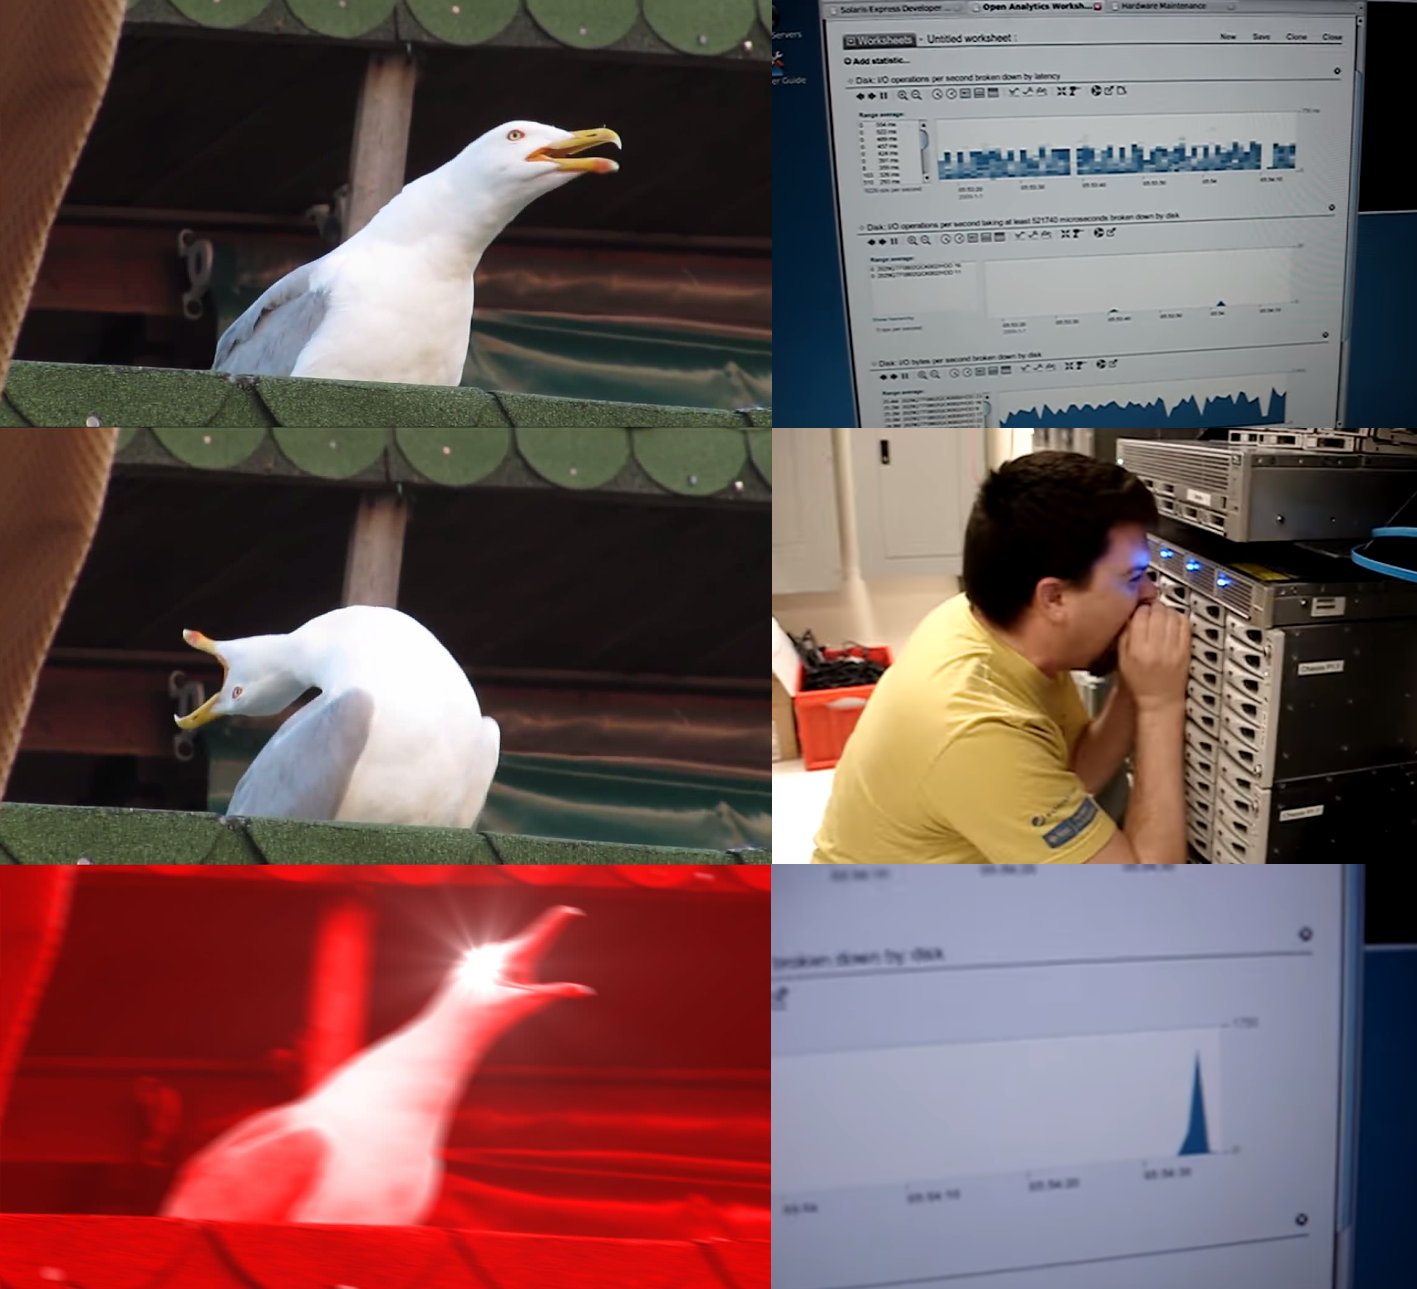
\includegraphics[height=\textheight]{img/meme.png}
		\end{flushright}
		\end{column}
	\end{columns}

\end{frame}
	\section{Доп. Материалы}
\subsection{Микробенчмаркинг}

\begin{frame}[fragile]{Функции, спасающие от слишком умного компилятора}
	\begin{enumerate}
		\item Помогает сохранить какой-то объект, не дать компилятору в ходе оптимизации избавиться от объекта:
\begin{lstlisting}
    static void escape(void *p) {
        asm volatile ("" : : "g"(p) : "memory");
    }
\end{lstlisting}

		\item Похожая функция, указывающая, что в момент исполнения возможна запись в любую область памяти, что помогает не дать компилятору избавиться от \enquote{бесполезных} операторов:
\begin{lstlisting}
    static void clobber() {
        asm volatile ("" : : : "memory");
    }
\end{lstlisting}

	\end{enumerate}
\end{frame}

\begin{frame}[fragile]{Пример кода теста example.cpp}
	\tiny
\begin{lstlisting}
#include "benchmark.h"
#include <vector>

static void escape(void *p) { asm volatile ("" : : "g"(p) : "memory"); }
static void clobber() { asm volatile ("" : : : "memory"); }

static void bm_create(benchmark::State &state) {
   while (state.KeepRunning()) {
      std::vector<int> v;
      escape(&v);   
      (void) v;   } } BENCHMARK(bm_create);

static void bm_reserve(benchmark::State &state) {
   while (state.KeepRunning()) {
      std::vector<int> v;
      v.reserve(1);
      escape(v.data());   } } BENCHMARK(bm_reserve);

static void bm_push_back(benchmark::State &state) {
   while (state.KeepRunning()) {
      std::vector<int> v;
      escape(v.data());
      v.push_back(42);
      clobber();   } } BENCHMARK(bm_push_back);

BENCHMARK_MAIN();
\end{lstlisting}
\end{frame}

\begin{frame}[fragile]{Как скомпилировать для Google Benchmark правильно?}
	\begin{itemize}
		\item -O2 или -O3 флаг, ибо в реальности ваше приложение будет компилироваться с применением оптимизаций, а значит тестировать надо уже с ними (и с ними же бороться).
		\item -fno-omit-frame-pointer -- позволяет сохранять границы кадров стека, что требуется для адекватного отображения результата профилирования в perf report
	\end{itemize}
	Итоговый минимальный makefile:
	\tiny
\begin{lstlisting}
   example: example.cpp
       g++ example.cpp -L. -lbenchmark -lpthread -O3 -fno-omit-frame-pointer -o example
\end{lstlisting}

	\normalsize
	На всякий случай: в системе должна быть установлена, либо находиться рядом библиотека pthread, собственно библиотека benchmark.a, а так же ее заголовочный файл benchmark.h.
\end{frame}

\begin{frame}[fragile]{Запуск теста и просмотр результата}
	\begin{enumerate}
		\item Используем perf record для записи результата:
\begin{lstlisting}
   perf record -g ./example
\end{lstlisting}
		\item Используем perf report для удобного просмотра результирующего дерева вызовов функций (пробелы после запятых не нужны!):
\begin{lstlisting}
   perf report -g "graph,0.5,caller"
\end{lstlisting}
	\end{enumerate}
	С интерфейсом предлагается разобраться самостоятельно, основываясь на предложенном видео выступления Чендлера. Стоит отметить, что при повторном просмотре ассемблерного кода perf может отматываться в самый низ ассемблера, т.о. требуется просто прокрутить экран вверх.
\end{frame}

\subsection{Память}
\begin{frame}[fragile]{Профилирование по памяти}
	Для записи выделения и освобождения памяти, а так же проблем связанных с данными процессами используется программа heaptrack. Чтобы явным образом ее опробовать требуется, соответственно, использовать операторы new и delete в коде. Запустить профилирование можно следующей командой:
\begin{lstlisting}
   heaptrack ./example
\end{lstlisting}
	Для просмотра результатов рекомендуется использовать утилиту heapsort\_gui.
	\begin{center}
		\includegraphics[width=.9\textwidth]{img/heaptrack_gui.png}
	\end{center}
\end{frame}

\subsection{FlameGraph}
\begin{frame}{FlameGraph -- наглядное отображение результатов профилирования}
	\begin{itemize}
		\item Основное:
		\begin{itemize}
			\item снизу вверх располагаются кирпичики-блоки функции в порядке уровня вложенности
			\item блоки вызванных функций располагаются строго на блоках их вызвавших
			\item на одном уровне блоки расположены по ширине соответственно использованию рассматриваемого ресурса
		\end{itemize}
		\item Нужные perl-скрипты располагаются в репозитории \href{https://github.com/brendangregg/FlameGraph}{\beamerbutton{GitHub}}
		\begin{itemize}
			\item stackcollapse-perf.pl -- для работы со срезами стека из perf
			\item flamegraph.pl -- для преобразования полученной из предыдущего скрипта структуры данных интерактивного svg-изображения с искомым флеймграфом.
		\end{itemize}
	\end{itemize}
\end{frame}

\begin{frame}[fragile]{Построение FlameGraph-а}
	\begin{enumerate}
		\item Сохраняем в директорию с результатами профилирования perf.data вышеупомянутые perl-скрипты. Не забываем дать им возможность исполняться, выполнив chmod +x на файлах скриптов.
		\item Получаем срезы стека из perf:
\scriptsize\begin{lstlisting}
   perf script > perf.script 
\end{lstlisting}\normalsize
		\item Обрабатываем первым скриптом:
\scriptsize\begin{lstlisting}
   ./stackcollapse-perf.pl perf.script > perf.folded
\end{lstlisting}\normalsize
		\item Получаем svg-файл вторым скриптом:
\scriptsize\begin{lstlisting}
   ./flamegraph.pl perf.folded > example.svg
\end{lstlisting}\normalsize
	\end{enumerate}
	\vspace{-0.5cm}
	\begin{center}
			\includegraphics[height=1.8cm]{img/flamegraph.png}
	\end{center}
\end{frame}


\end{document}